% file: circular-queue.tex
% Code template from https://tex.stackexchange.com/a/18372/23098

\documentclass[tikz]{standalone}

\begin{document}
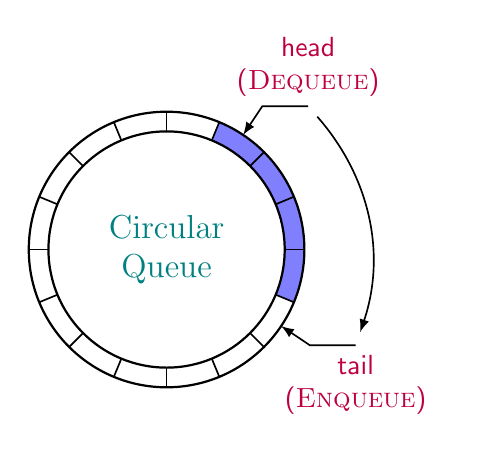
\begin{tikzpicture}[>=latex,font=\sffamily,semithick,scale=1.75]
    \fill [blue!50] (0,0) -- (67.5:1) arc [end angle=-22.5, start angle=67.5, radius=1] -- cycle;
    \draw [thick] (0,0) circle (1);
    \foreach \angle in {90,67.5,...,-67.5}
        \draw (\angle:1) -- (\angle-180:1);

    \node [circle, thick, fill=white, draw=black, align=center, minimum size=3cm, font = \large] 
      at (0,0) {\textcolor{teal}{Circular} \\ {\textcolor{teal}{Queue}}};

    \draw [<-] (56.25:1) -- (56.25:1.25) -- +(.333,0)
      node [inner xsep=.333cm, align = center, above, purple] (Head) {head \\ (\textsc{Dequeue})};
    \draw [<-] (-33.75:1) -- (-33.75:1.25) -- +(.333,0)
      node [inner xsep=.333cm, align = center, below, purple] (Tail) {tail \\ (\textsc{Enqueue})};

    \draw [->,shorten >=5pt,shorten <=5pt] (Head.south) to [bend left] 
        node [midway, sloped, above, allow upside down] {}
    (Tail.north);
\end{tikzpicture}
\end{document}
